%% Article version of the undergraduate thesis (TG, ITA):
%% "Hawkes Process Estimation on High-Frequency Cryptocurrency Data via Neural Networks".
%% Every number below is taken from thesis/tg (and the fragments it inputs from thesis/latex)
%% or from docs/decisions/008 and 009. Build instructions: thesis/paper/README.md.
\documentclass[preprint,12pt,authoryear]{elsarticle}

\usepackage[utf8]{inputenc}
\usepackage{amsmath,amssymb}
\usepackage{booktabs}
\usepackage{graphicx}
\usepackage{microtype}
\usepackage[a4paper,hmargin=2.5cm,vmargin=2.8cm]{geometry}
\usepackage[hidelinks]{hyperref}

\graphicspath{{../build/figures/}}

\newcommand{\aself}{\alpha_{\mathrm{s}}}
\newcommand{\across}{\alpha_{\mathrm{c}}}
\newcommand{\E}{\mathbb{E}}
\DeclareMathOperator{\softplus}{softplus}

\myfooter[L]{Draft for advisor review, \today}
\hypersetup{pdftitle={Neural estimation of a bivariate Hawkes process on high-frequency
  cryptocurrency data: a reproduction of Lee (2023) and a test of attention},
  pdfauthor={João Matheus Del Vecchio França Barbosa; Mauri Aparecido de Oliveira}}

\begin{document}

\begin{frontmatter}

\title{Neural estimation of a bivariate Hawkes process on high-frequency
cryptocurrency data: a reproduction of \texorpdfstring{\citet{lee2023}}{Lee (2023)} and a test of attention}

% TODO: confirm authorship order with advisor
\author{Jo\~{a}o Matheus Del Vecchio Fran\c{c}a Barbosa\corref{cor}}
\author{Mauri Aparecido de Oliveira}
\cortext[cor]{Corresponding author.}
\address{Instituto Tecnol\'{o}gico de Aeron\'{a}utica (ITA), S\~{a}o Jos\'{e} dos
Campos, SP, Brazil}

\begin{abstract}
We reproduce and extend the amortized neural estimation of a symmetric bivariate
exponential Hawkes process proposed by \citet{lee2023}, using mid-price changes of Binance
BTCUSDT and ETHUSDT perpetual futures on a 100~ms grid. Under a frozen synthetic protocol
(100,000 paths of 1,000 events, five seeds per network), the paper's LSTM attains a macro
MSE of 0.0196 and a Transformer encoder 0.0237 ($p=0.19$ across seeds): attention does not
improve accuracy. The maximum likelihood estimator (MLE) has a macro MSE of 0.506, driven by
the 1\% of paths in which the decay rate is weakly identified; on a typical path it is as
accurate as the networks and, with an analytic gradient, costs about 10~ms, the same order
as a network at batch size one. On real windows, the Hawkes model beats a Poisson process in
99.8\% of the cases but leaves serial dependence in the residuals, and its estimates lie
outside the synthetic prior, with null cross-excitation. Fine-tuned from the synthetic
weights on MLE labels of real windows, the networks reach a test macro MSE of 0.044 (LSTM,
selected on validation) and 0.040 (Transformer), against 0.218 for the label mean. The
Hawkes volatility implied by the MLE ranks windows like realized volatility (Spearman 0.78);
the network's keeps the level but not the ranking (0.28). A pre-registered addendum, evaluated
on a new week, shows that the selected LSTM was undertrained (a longer budget lowers its loss
by 20\%, from 0.026 to 0.021) and that averaging the LSTM and the Transformer is the most
accurate estimator (0.020); it also shows that the 100~ms grid makes the MLE recover only
about 58\% of the continuous-time decay rate. Pretraining on a prior built from the real
labels and simulated on the same grid cuts the loss on a second new week (March 2024) by 63\%
(0.109 to 0.040), the largest out-of-sample gain of this work. Trained on the true parameters
of gridded paths, the LSTM undoes the grid bias in simulation, but the correction does not
transfer safely to real windows.
\end{abstract}

\begin{keyword}
Hawkes processes \sep high-frequency data \sep cryptocurrencies \sep amortized inference
\sep LSTM \sep Transformer\break
\textit{JEL classification:} C13, C45, C58
\end{keyword}

\end{frontmatter}

%% ===========================================================================================
\section{Introduction}
\label{sec:intro}

At short time scales a price is a sequence of discrete events, and these events cluster:
a change tends to be followed by further changes, so that calm periods alternate with
bursts. The homogeneous Poisson process cannot represent this dependence. The Hawkes
process \citep{hawkes1971,hawkes1971b}, whose intensity rises after each event and then
decays, can, and it has become a reference model of market microstructure
\citep{bowsher2007,bacry2013,bacry2015,hawkes2018}. Its branching ratio measures how much of
the activity is endogenous \citep{filimonov2012,hardiman2013}, and its parameters determine
a model-implied volatility \citep{leeseo2017,lee2024}.

Estimation is usually done by maximum likelihood, which for exponential kernels is
$O(n)$ per evaluation \citep{ozaki1979} and asymptotically efficient \citep{ogata1978},
but requires an iterative optimization for every new window. \citet{lee2023} proposes to
pay a training cost once instead: an LSTM is trained on simulated paths and maps an observed
sequence directly to the four parameters of a symmetric bivariate Hawkes process of up- and
down-moves. This is amortized, simulation-based inference \citep{cranmer2020}, a strategy
also used for spatial and extreme-value models \citep{gerber2021,lenzi2023} and, recently,
for Hawkes processes observed only through counts \citep{lambe2025}. A different line of
work, the neural point processes \citep{du2016,mei2017,zuo2020,zhang2020,shchur2021}, uses
networks to model the intensity itself; our goal is narrower, namely to estimate the
interpretable parameters of a classical model.

\citet{lee2023} studied US equities with non-public NBBO data, left several protocol details
unspecified, and considered a single compact recurrent architecture. Crypto-assets are a
natural test bed: trading is continuous, best bid and offer data are public, and the market
differs structurally from equities \citep{makarov2020,he2022perpetual}. Hawkes models have
been fitted by MLE to jumps in one-minute crypto returns \citep{taddeo2024}; here we work at
the level of top-of-book events and with amortized neural estimation. We ask whether an
attention-based architecture can estimate the parameters of a bivariate Hawkes process on
cryptocurrency price changes with accuracy and stability equal to or better than Lee's LSTM,
while keeping inference faster than the MLE. Three hypotheses were registered before the
final run: (H1) Binance's public USD-M data yield sequences structurally equivalent to
Lee's inputs; (H2) the LSTM attains error of the same order as the MLE at substantially
lower latency; and (H3) attention improves error or robustness on sequences with
long-range dependence.

Our contributions are the following.
\begin{itemize}
  \item \emph{A controlled reproduction.} We re-implement simulation, MLE and the LSTM,
        document the gaps in \citet{lee2023}, and reproduce the paper's sampling
        distribution at its published parameter point.
  \item \emph{A sharper reading of the synthetic comparison.} Per-parameter $R^2$, paired
        per-path tests and a diagnosis of the MLE show that the networks' advantage in
        aggregate MSE comes from a small set of weakly identified paths and from shrinkage
        toward the training prior, not from higher accuracy on a typical path; with an
        efficient MLE, the speed gain reported by Lee is not reproduced at batch size one.
  \item \emph{A negative result for attention on synthetic data.} A Transformer encoder
        trained under the same protocol does not outperform the LSTM in any regime of the
        branching ratio.
  \item \emph{A pre-registered empirical stage.} We characterize the mid-price events of
        BTCUSDT and ETHUSDT, separate the effect of the 100~ms grid from model
        misspecification in goodness-of-fit tests, train networks on MLE labels of real
        windows (from scratch, fine-tuned and zero-shot) with a test block opened once,
        check robustness on a different month, and compare the implied Hawkes volatility
        with realized volatility.
\end{itemize}

Section~\ref{sec:model} presents the model and the estimators, Section~\ref{sec:data} the
data and Section~\ref{sec:design} the experimental design. Section~\ref{sec:results} reports
the results, Section~\ref{sec:discussion} discusses them and Section~\ref{sec:conclusion}
concludes.

%% ===========================================================================================
\section{Model and estimators}
\label{sec:model}

\subsection{Symmetric bivariate Hawkes process}

Let $N_1$ and $N_2$ count the up- and down-moves of the mid-price, with event times
$t^1_k$ and $t^2_k$. The symmetric exponential model of \citet{lee2023} has intensities
\begin{equation}
\lambda_i(t)=\mu+\sum_{t^i_k<t}\aself e^{-\beta(t-t^i_k)}
  +\sum_{t^j_k<t}\across e^{-\beta(t-t^j_k)},\qquad i\neq j\in\{1,2\},
\label{eq:intensity}
\end{equation}
with baseline $\mu$, self-excitation $\aself$, cross-excitation $\across$ and decay $\beta$.
Dominant cross-excitation describes short-term reversion (an up-move followed by a
down-move) and dominant self-excitation describes persistence of direction
\citep{bacry2013}. The kernel mass matrix has largest eigenvalue
\begin{equation}
g=\frac{\aself+\across}{\beta},
\end{equation}
the branching ratio; $g<1$ is required for stationarity, and cascades lengthen as $g\to1$
\citep{hardiman2013,filimonov2012}. The stationary rate of each direction is
$\Lambda=\mu/(1-g)$.

\subsection{Maximum likelihood}

For $\theta=(\mu,\aself,\across,\beta)$ and horizon $T$, the log-likelihood is
\begin{equation}
\ell(\theta)=\sum_k\log\lambda_{c_k}(t_k)-\sum_{i=1}^{2}\int_0^T\lambda_i(u)\,\mathrm du,
\end{equation}
where $c_k$ is the type of the $k$-th event. With exponential kernels the sums over the past
obey a first-order recursion, so $\ell$ and its gradient cost $O(n)$ \citep{ozaki1979}. We
parametrize $(\mu,\aself,\across,d)=\softplus(z)$ and set $\beta=\aself+\across+d$, which
enforces $g<1$, and maximize with L-BFGS-B from five starting points: one based on the
empirical event rate and four random perturbations in the unconstrained space. The MLE never
receives the true parameter. The gradient is analytic and the recursions are solved as
bidiagonal linear systems.

Consistency and efficiency are asymptotic. With 1,000 events and weak excitation, the kernel
barely moves the intensity and the likelihood is nearly flat in $\beta$; as
$\aself+\across\to0$, $\beta$ is not identified. Near criticality, the mean rate $2\mu/(1-g)$
is well determined but $\mu$ and $g$ separately are not. Both effects matter below.

\subsection{Neural estimators}

Each event is encoded as $(\log(1+\Delta t),\,s)$, with $\Delta t$ the inter-arrival time and
$s=\pm1$ the direction. Both networks share the output head: a softplus produces
$\mu,\aself,\across,d>0$ and $\beta=\aself+\across+d$, so every estimate satisfies $g<1$, as
in Lee's robust variant. The loss is the MSE on the original parameter scale.

The \emph{LSTM} follows \citet{lee2023}: two LSTM layers of 12 units \citep{hochreiter1997}
followed by a dense layer, 2,068 trainable parameters. The \emph{Transformer} is an encoder
\citep{vaswani2017} with a linear projection from 2 to 32 dimensions, sinusoidal positional
encoding, two post-LN layers with four heads of dimension eight, a feed-forward block
$32\to128\to32$, dropout 0.1 and temporal mean pooling, for 25,700 trainable parameters. Its
attention cost is quadratic in the sequence length, and the post-LN variant usually benefits
from learning-rate warm-up \citep{xiong2020}, which we did not use.

Training on pairs $(\theta_i,x_i)$ with $\theta_i\sim\pi$ and squared loss minimizes the Bayes
risk under the prior $\pi$, whose minimizer is the posterior mean $\E_\pi[\theta\mid x]$
\citep{lehmann1998,sainsburydale2024}. On a test set drawn from
$\pi$, no estimator has lower average MSE than the posterior mean, so beating the MLE there
is expected and is not evidence of frequentist superiority. Also, the network does not
extrapolate: its estimates shrink toward the high-density region of $\pi$, so data outside
the support of the prior produce biased estimates.

\subsection{Hawkes volatility}

Let $J$ be the absolute log return of an event, assumed i.i.d., and let $a_s=\aself/\beta$
and $a_c=\across/\beta$. For the symmetric model the long-run variance of the log price per
unit time is \citep{bacry2013}
\begin{equation}
\sigma_H^2=2\Lambda\left[\operatorname{Var}(J)+\frac{\E[J]^2}{(1-a_s+a_c)^2}\right],
\qquad \Lambda=\frac{\mu}{1-a_s-a_c}.
\label{eq:hawkes-vol}
\end{equation}
The factor $(1-a_s+a_c)^{-2}$ makes persistence ($a_s>a_c$) amplify variance and reversion
damp it. We compare $\sigma_H$, scaled by the square root of the window duration, with the
realized volatility of the log mid-price \citep{andersen2003,barndorff2002}.

%% ===========================================================================================
\section{Data}
\label{sec:data}

The best bid and ask are needed to reconstruct the mid-price, and the official Binance
archive provides a historical \texttt{bookTicker} stream for USD-M futures but not for
spot.\footnote{Binance Public Data, \url{https://data.binance.vision}.} We therefore use the
BTCUSDT and ETHUSDT perpetual futures. Each downloaded file is recorded with its SHA-256, and audits check for
positive prices, bid not above ask, time ordering and duplicate timestamps. Following
\citet{lee2023}, updates are reduced to a 100~ms grid keeping the last state of each cell,
and an event is a change of the mid-price; the event type is its direction and the mark is
its size in ticks.

The primary window is 15--28 January 2024; all 56 expected files (14 days, two symbols,
\texttt{bookTicker} and \texttt{aggTrades}) were present. It is cut into non-overlapping
windows of 1,000 events and split chronologically by day into calibration (15--22 January,
1,063 windows), validation (23--25 January, 476) and test (26--28 January, 274). The week of
23--29 October 2023 is a robustness window, used neither for training nor for selection
(Table~\ref{tab:data}).

\begin{table}[t]
\centering
\caption{Data coverage and characteristics of the mid-price events. Panel B uses the
calibration block (15--22 January 2024).}
\label{tab:data}
\small
\begin{tabular}{lrr}
\toprule
\multicolumn{3}{l}{\emph{Panel A: coverage}}\\
 & Primary (Jan.\ 2024) & Robustness (Oct.\ 2023)\\
\midrule
Symbol-days & 28 & 14\\
Events, BTCUSDT & 887,803 & 652,773\\
Events, ETHUSDT & 939,101 & 635,579\\
Events, total & 1,826,904 & 1,288,352\\
Windows of 1,000 events & 1,813 & 1,281\\
\midrule
\multicolumn{3}{l}{\emph{Panel B: event characteristics}}\\
 & BTCUSDT & ETHUSDT\\
\midrule
Events & 529,278 & 540,164\\
Fraction of up-moves & 49.4\% & 49.5\%\\
Repeats the previous direction & 76.0\% & 75.7\%\\
Median inter-arrival time & 0.3 s & 0.3 s\\
Inter-arrivals equal to the grid step & 39.5\% & 37.3\%\\
Median / 90th percentile jump (ticks) & 15.5 / 48 & 10 / 29\\
One-tick jumps & 9.7\% & 12.6\%\\
\bottomrule
\end{tabular}
\end{table}

Three features set these data apart from Lee's equities. About 76\% of the changes repeat
the previous direction, which points to persistence rather than reversion. The median jump
is 10 to 15 ticks and only 10--13\% are one tick, so at this scale the contracts behave as
small-tick assets. And 37--39\% of the inter-arrival times equal the grid step: the
sampling discretizes time, whereas the model and the simulations are in continuous time.

%% ===========================================================================================
\section{Experimental design}
\label{sec:design}

Every decision is labelled as published information (R1), a reconstruction of a gap in the
paper (R2), an adaptation to crypto (A1) or an extension (E1, the Transformer). The
protocols below were fixed in decision records before the corresponding test sets were read.

\subsection{Synthetic protocol}

Paths are simulated by thinning \citep{ogata1981} from an empty history, the same
assumption as in the likelihood, and have exactly 1,000 events. The frozen experiment has
75,000 training, 10,000 validation and 15,000 test paths. Parameters are drawn with
$\mu\in[0.2,0.6]$, $\beta\in[0.8,2.0]$, self-excited fraction $\aself/(\aself+\across)
\in[0.2,0.8]$, and $g$ balanced across three strata: low $[0.10,0.35)$, intermediate
$[0.35,0.70)$ and near-critical $[0.70,0.95]$. Lee does not publish his ranges, so these are
R2. Each network is trained with five seeds, Adam with learning rate $10^{-3}$, at most 300
epochs and early stopping with patience 30 on the validation loss (Table~\ref{tab:training}).
There was no hyperparameter search for either network.

\begin{table}[t]
\centering
\caption{Synthetic training configuration and cost (five seeds per network, Apple Silicon
with MPS).}
\label{tab:training}
\small
\begin{tabular}{lrr}
\toprule
 & LSTM (R1/R2) & Transformer (E1)\\
\midrule
Trainable parameters & 2,068 & 25,700\\
Effective batch & 64 & 8 (4 with accumulation)\\
Best epoch (per seed) & 165, 164, 193, 239, 299 & 73, 42, 38, 60, 44\\
Training time per seed & 5.4--14.8 h & 16.6--28.8 h\\
Total time (5 seeds) & 41 h & 110 h\\
\bottomrule
\end{tabular}
\end{table}

We report per-parameter and macro MSE, median absolute error, the MSE of $g$, validity and
MLE convergence. Because the parameters have different scales, we also report the $R^2$ of
each parameter relative to the prior mean. Networks are compared in two ways: across seeds
(Welch and Mann--Whitney tests on five seeds), which measures training variability
\citep{bouthillier2021}, and across test paths (paired difference of the ensembles with a
bootstrap interval and a Wilcoxon test), which measures the accuracy of the trained models
\citep{efron1993,diebold1995}. The per-path analysis was added after the aggregate results
were known and is therefore post hoc; it uses the frozen checkpoints, which reproduce the
reported MSE to a relative difference of $10^{-8}$, and changes nothing in the protocol.

\paragraph{Fixed point} To compare with the sampling-distribution table of \citet{lee2023},
2,000 paths are simulated at the published point $\mu=0.3$, $\aself=0.4$, $\across=0.7$,
$\beta=1.5$, which lies inside our prior. The networks are applied without retraining, and the MLE
is run both with our heuristic starts and with Lee's initialization at the true value.

\subsection{Empirical protocol}

On real data there is no true parameter, so the empirical stage asks three narrower
questions, fixed before the test block was opened: does the Hawkes model describe the
windows, can a network reproduce the MLE on real windows, and does the estimate imply a
volatility consistent with the realized one?

\paragraph{Goodness of fit} With the MLE of each calibration window, the time-rescaled
residuals of each dimension are tested against $\mathrm{Exp}(1)$ by Kolmogorov--Smirnov (KS)
and for serial dependence by Ljung--Box at 10 lags \citep{ogata1988,brown2002}, and the Hawkes
model is compared with a homogeneous bivariate Poisson process by likelihood ratio and AIC.
Two controls separate the grid from misspecification: real times jittered uniformly inside
their 100~ms cell, with the MLE refitted; and paths simulated from each fitted model, kept in
continuous time or mapped to the grid (one event per cell) and jittered in the same way.

\paragraph{Networks on real windows (scope A)} Each window is labelled with its MLE. Both
architectures are trained on the calibration labels with the loss, batch, epoch limit and
patience of the synthetic protocol, in two variants, each with the five protocol seeds: from
scratch (learning rate $10^{-3}$) and fine-tuned from the synthetic weights of the same seed
(learning rate $10^{-4}$). Two references need no training: the synthetic networks as they
are (zero-shot) and the mean of the training labels, the best constant predictor. The
selected variant is the one whose five-seed ensemble has the lowest validation macro MSE.
The test block is labelled and evaluated once, after the selection, with the stored weights;
all variants are reported. The October week is labelled and evaluated in the same way. The
machine budget was capped at 30~h; training used 3.0~h.

\paragraph{Volatility} Equation~\eqref{eq:hawkes-vol} is evaluated per window with the
MLE and with the selected network, and compared with the realized volatility sampled every
$\Delta\in\{0.1,1,5,10,30\}$~s. The metrics, fixed before the test was opened, are the median
ratio $\sigma_H/\sigma_{RV}$ and the Spearman correlation across windows, with $\Delta=10$~s
as the main horizon.

%% ===========================================================================================
\section{Results}
\label{sec:results}

\subsection{Reproduction at the published fixed point}

Table~\ref{tab:e2} reproduces the qualitative pattern of \citet{lee2023}. The MLE is nearly
unbiased, with standard deviations about $\sqrt2$ times Lee's, as expected for paths of half
the length. The networks shrink $\aself$ and $\across$ toward the centre of the prior in
exchange for lower variance, as in the paper. The two MLE versions produce identical
estimates, so initialization at the truth does not explain the MLE's accuracy at this
well-identified point ($g\approx0.73$). The macro MSE is 0.0103 for the MLE and 0.0111 for
the LSTM ensemble.

\begin{table}[t]
\centering
\caption{Sampling distribution at the fixed point of \citet{lee2023}
($\mu=0.3$, $\aself=0.4$, $\across=0.7$, $\beta=1.5$): mean and standard deviation over
2,000 paths of 1,000 events. Lee's rows use 100,000 paths of 2,000 steps.}
\label{tab:e2}
\footnotesize
\setlength{\tabcolsep}{4pt}
\begin{tabular}{lrrrrrrrr}
\toprule
 & \multicolumn{2}{c}{$\mu$} & \multicolumn{2}{c}{$\aself$} & \multicolumn{2}{c}{$\across$}
 & \multicolumn{2}{c}{$\beta$}\\
\cmidrule(lr){2-3}\cmidrule(lr){4-5}\cmidrule(lr){6-7}\cmidrule(lr){8-9}
Estimator & Mean & SD & Mean & SD & Mean & SD & Mean & SD\\
\midrule
LSTM (5-seed ensemble) & 0.3044 & 0.0365 & 0.4950 & 0.0536 & 0.6245 & 0.0608 & 1.5318 & 0.1436\\
Transformer (5-seed ensemble) & 0.2957 & 0.0388 & 0.5280 & 0.0561 & 0.6055 & 0.0620 & 1.5308 & 0.1541\\
MLE, heuristic (5 starts) & 0.3065 & 0.0370 & 0.3956 & 0.0728 & 0.7075 & 0.0859 & 1.5156 & 0.1642\\
MLE, started at the truth & 0.3065 & 0.0370 & 0.3956 & 0.0728 & 0.7075 & 0.0859 & 1.5156 & 0.1642\\
\citet{lee2023}, network & 0.3151 & 0.0358 & 0.4429 & 0.0661 & 0.5733 & 0.0697 & 1.5736 & 0.1364\\
\citet{lee2023}, MLE & 0.3036 & 0.0314 & 0.3988 & 0.0500 & 0.7024 & 0.0608 & 1.5078 & 0.1145\\
\bottomrule
\end{tabular}
\end{table}

\subsection{Synthetic comparison: LSTM, Transformer and MLE}

Table~\ref{tab:synthetic} summarizes the frozen test set. All estimators produce valid
parameters on every path and the MLE converges on all of them (median of 14 iterations).
The LSTM's mean macro MSE is 17.2\% lower than the Transformer's, but with five seeds each
the difference is not significant (Welch $p=0.19$; Mann--Whitney $p=0.056$) and the
confidence intervals overlap. Part of the seed dispersion comes from the LSTM, which showed
two convergence levels across seeds, with one seed stopping at the 300-epoch limit while
still improving.

\begin{table}[t]
\centering
\caption{Frozen synthetic test set (15,000 paths of 1,000 events). Macro MSE overall (with
95\% $t$ interval across five seeds) and by regime of $g$; MSE per parameter. Network rows
are means over seeds.}
\label{tab:synthetic}
\small
\setlength{\tabcolsep}{4.5pt}
\begin{tabular}{lrcrrrr}
\toprule
 & \multicolumn{2}{c}{Macro MSE} & \multicolumn{3}{c}{Macro MSE by regime of $g$} & \\
\cmidrule(lr){2-3}\cmidrule(lr){4-6}
Estimator & Mean & 95\% CI & Low & Interm. & Near-crit. & MSE of $g$\\
\midrule
LSTM & 0.0196 & [0.0133, 0.0260] & 0.0199 & 0.0156 & 0.0233 & 0.0018\\
Transformer & 0.0237 & [0.0191, 0.0283] & 0.0222 & 0.0190 & 0.0299 & 0.0021\\
MLE & 0.5062 & -- & 1.4806 & 0.0168 & 0.0212 & 0.0023\\
\midrule
 & \multicolumn{6}{l}{MSE by parameter: $\mu$ / $\aself$ / $\across$ / $\beta$}\\
\midrule
LSTM & \multicolumn{6}{l}{0.0023 / 0.0162 / 0.0166 / 0.0434}\\
Transformer & \multicolumn{6}{l}{0.0024 / 0.0209 / 0.0212 / 0.0503}\\
MLE & \multicolumn{6}{l}{0.0101 / 0.0061 / 0.0062 / 2.0023}\\
\bottomrule
\end{tabular}
\end{table}

The MLE's aggregate error is almost entirely $\beta$ (98.9\% of its sum of squared errors),
and its macro MSE in the low-$g$ regime is 88 times that of the intermediate regime. Outside
the low regime the MLE is competitive: 0.0168 against 0.0156 (LSTM) and 0.0190
(Transformer) in the intermediate regime, and 0.0212 against 0.0233 and 0.0299 near
criticality. It also has the lowest MSE of the three for $\aself$ and $\across$.

The post hoc per-path analysis (Table~\ref{tab:posthoc}) explains the gap. First, 1\% of the
paths, almost all with low $g$, carry 94.4\% of the MLE's squared error in $\beta$
(Fig.~\ref{fig:beta}). This is an identification failure, not a numerical one: on each of the
300 worst paths the log-likelihood at the estimate exceeds that at the true parameter
(median gain 2.80), and refitting 100 of them with 20 starts barely changes the result.
Second, on the typical path the MLE is as good as the networks: its median standardized loss
equals the LSTM's overall (0.149 versus 0.151) and is lower in the intermediate and
near-critical regimes, and its $R^2$ for $\aself$ and $\across$ is 0.90, against 0.82 and
0.81 for the LSTM. Third, path by path, the LSTM ensemble beats the Transformer
ensemble in every regime, including the near-critical one, where long memory should favour
attention.

\begin{table}[t]
\centering
\caption{Post hoc analysis of the synthetic test set. Panel A: $R^2$ relative to the prior
mean, macro median absolute error (AE) and MSE of $g$ (network ensembles). Panel B: paired
per-path comparison of the mean standardized squared error; median loss of A and B, share
of paths where A is better, and bootstrap 95\% CI of the mean difference A$-$B (negative
favours A).}
\label{tab:posthoc}
\footnotesize
\setlength{\tabcolsep}{5pt}
\begin{tabular}{lrrrrrr}
\multicolumn{7}{l}{\emph{Panel A: accuracy relative to the prior mean}}\\
\toprule
Estimator & $R^2_\mu$ & $R^2_{\aself}$ & $R^2_{\across}$ & $R^2_\beta$ & Median AE & MSE of $g$\\
\midrule
Prior mean & $-$0.01 & 0.00 & $-$0.01 & 0.01 & 0.1908 & 0.0670\\
MLE & 0.24 & 0.90 & 0.90 & $-$15.64 & 0.0674 & 0.0023\\
LSTM (ensemble) & 0.84 & 0.82 & 0.81 & 0.65 & 0.0680 & 0.0017\\
Transformer (ensemble) & 0.84 & 0.74 & 0.73 & 0.61 & 0.0765 & 0.0019\\
\bottomrule
\end{tabular}

\vspace{1.2ex}
\begin{tabular}{llrrrr}
\multicolumn{6}{l}{\emph{Panel B: paired comparison per path}}\\
\toprule
A $\times$ B & Regime & Med.\ A & Med.\ B & A better & 95\% CI (A$-$B)\\
\midrule
LSTM $\times$ Transformer & all & 0.151 & 0.187 & 70.2\% & [$-$0.051, $-$0.047]\\
 & low $g$ & 0.112 & 0.131 & 61.1\% & [$-$0.021, $-$0.016]\\
 & intermediate $g$ & 0.127 & 0.164 & 72.8\% & [$-$0.045, $-$0.041]\\
 & near-critical $g$ & 0.237 & 0.304 & 76.7\% & [$-$0.089, $-$0.081]\\
\midrule
LSTM $\times$ MLE & all & 0.151 & 0.149 & 48.8\% & [$-$9.394, $-$0.809]\\
 & low $g$ & 0.112 & 0.199 & 63.5\% & [$-$26.977, $-$2.225]\\
 & intermediate $g$ & 0.127 & 0.100 & 40.1\% & [$-$0.040, $-$0.009]\\
 & near-critical $g$ & 0.237 & 0.183 & 42.7\% & [$-$0.467, $-$0.277]\\
\midrule
Transformer $\times$ MLE & all & 0.187 & 0.149 & 43.5\% & [$-$9.376, $-$0.782]\\
 & low $g$ & 0.131 & 0.199 & 59.4\% & [$-$27.686, $-$2.207]\\
 & intermediate $g$ & 0.164 & 0.100 & 34.2\% & [0.002, 0.035]\\
 & near-critical $g$ & 0.304 & 0.183 & 36.7\% & [$-$0.374, $-$0.195]\\
\bottomrule
\end{tabular}
\end{table}

\begin{figure}[t]
\centering
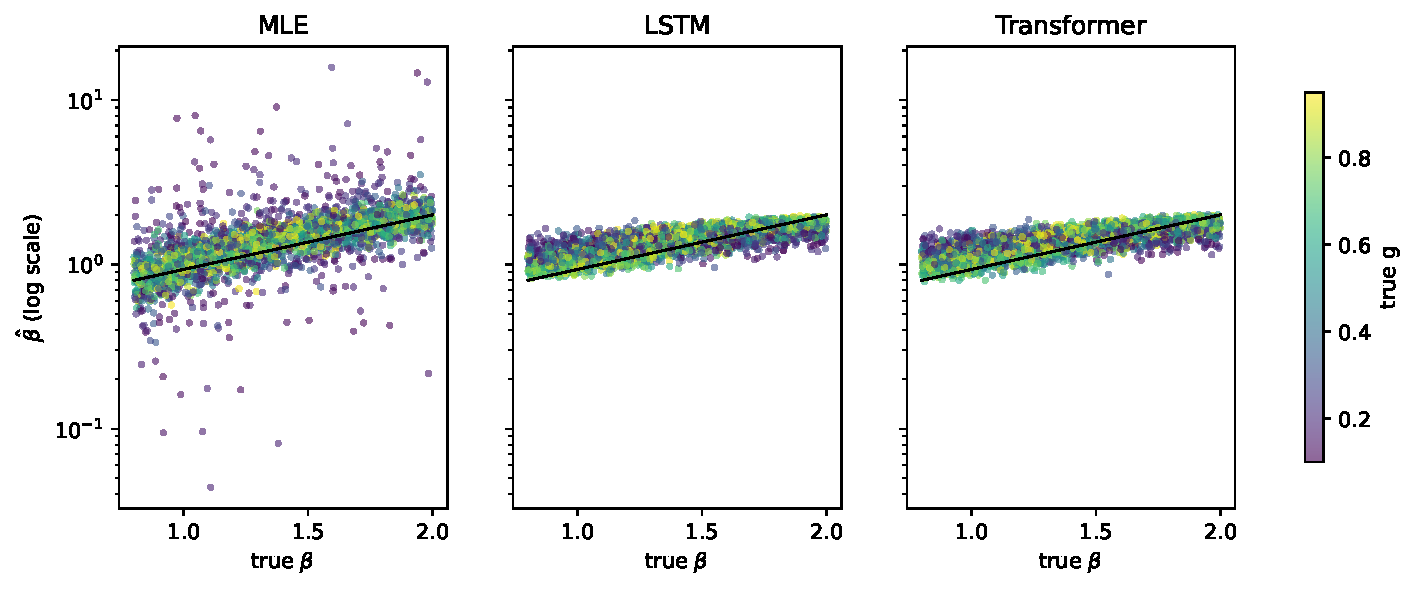
\includegraphics[width=0.9\linewidth]{posthoc_beta_verdadeiro_vs_estimado_en.pdf}
\caption{True versus estimated $\beta$ on 3,000 synthetic test paths (logarithmic scale;
colour is the true $g$). The networks shrink toward the centre of the prior; the MLE is
unbiased over most of the domain but produces extreme values when $g$ is low.}
\label{fig:beta}
\end{figure}

Paired intervals for network minus MLE are negative overall even though the medians are
equal, because the mean is dominated by the few extreme MLE errors. Panel~A makes the same
point: the networks never leave $[0.8,2.0]$ for $\beta$, which bounds their worst case,
while the MLE's $R^2_\beta$ is $-15.64$.

\paragraph{Computational cost} During the final run, the MLE was timed at 105~ms per path
while competing with neural training for the machine. A controlled benchmark of the same code,
which reproduces the 15,000 recorded estimates exactly, gives the values in
Table~\ref{tab:cost}. With an analytic gradient and a linear recursion, the MLE costs a few
milliseconds, the same order as a network at batch size one; the network advantage of about
150 times reported by \citet{lee2023} is not reproduced. The networks' cost advantage appears
in batched inference, above all for the LSTM.
Lee does not describe his MLE. Fitting the same paths at his fixed point with implementations
that differ in one factor at a time (Table~\ref{tab:cost-variants}) gives the same estimates in
every variant and isolates the likelihood as the dominant cost: a double sum over pairs of events
costs about 90 times as much as the recursion at 2,000 events, while a numerical gradient and
Nelder--Mead add about a factor of five each. Lee's 1,763~ms falls between the two vectorized
double-sum variants, so the reported ratio most likely reflects a likelihood computed without the
recursion.

\begin{table}[t]
\centering
\caption{Cost per path of 1,000 events in a controlled benchmark.}
\label{tab:cost}
\small
\begin{tabular}{lr}
\toprule
Estimator and execution mode & Time per path\\
\midrule
MLE, 5 starts, one core & 9.6 ms\\
MLE, 1 start, one core & 2.2 ms\\
MLE, 5 starts, 4 processes (wall-clock) & 2.5 ms\\
LSTM, batch size one, CPU (1 thread) / MPS & 7.0 / 29.6 ms\\
Transformer, batch size one, CPU (1 / 10 threads) / MPS & 9.9 / 4.8 / 5.0 ms\\
LSTM, batch of 256, MPS & 0.07 ms\\
Transformer, batch of 32, MPS & 3.7 ms\\
\midrule
\citet{lee2023}: network / MLE & 12 / 1,763 ms\\
\bottomrule
\end{tabular}
\end{table}

\begin{table}[t]
\centering
\caption{Cost of one MLE fit by implementation, at the fixed point of \citet{lee2023}: median of
10 paths, one start at the true parameters, one core. The pure-Python double sum was timed for
one evaluation and multiplied by the number of evaluations of the vectorized Nelder--Mead fit.}
\label{tab:cost-variants}
\small
\begin{tabular}{llrr}
\toprule
Likelihood & Gradient and optimizer & 1,000 events & 2,000 events\\
\midrule
Recursion, vectorized & analytic, L-BFGS-B (this work) & 1.1 ms & 1.7 ms\\
Recursion, vectorized & numerical, L-BFGS-B & 5.4 ms & 8.3 ms\\
Recursion, Python loop & numerical, L-BFGS-B & 47 ms & 89 ms\\
Double sum, vectorized & numerical, L-BFGS-B & 176 ms & 711 ms\\
Double sum, vectorized & Nelder--Mead & 818 ms & 3,358 ms\\
Double sum, Python loop & Nelder--Mead (extrapolated) & 26 s & 105 s\\
\midrule
\multicolumn{3}{l}{\citet{lee2023}, implementation not described} & 1,763 ms\\
\bottomrule
\end{tabular}
\end{table}

\subsection{Real data: goodness of fit and the location of the estimates}
\label{sec:real-fit}

The MLE converged on all 1,063 calibration windows. Table~\ref{tab:diagnostics} and
Fig.~\ref{fig:diagnostics} summarize the residual diagnostics. The Hawkes model is far
better than a homogeneous Poisson process: the likelihood ratio rejects Poisson at 1\% in
99.8\% of the windows, with a median AIC difference of $-721$. It is not the data-generating
process, though. KS rejects in 70.3\% of the jittered real windows, but the grid alone makes
it reject in 47.7\% of the simulated controls, so only part of that is misspecification.
Ljung--Box keeps its nominal size on the simulated grid (4.7\%) and rejects in 47.1\% of the
jittered real windows: part of the clustering remains in the residuals, beyond what a single
exponential kernel absorbs. Jittering barely moves the estimates (median $\beta$ from 2.71
to 2.77; median $\aself$ from 1.34 to 1.36). Repeated once on the 274 test windows, after
the test was opened, the diagnostic shows the same pattern: Poisson is rejected in 100.0\%
of the windows (median AIC difference $-905$), and Ljung--Box rejects in 47.1\% of the
jittered real windows against 4.2\% in the simulated grid controls.

\begin{table}[t]
\centering
\caption{Residual diagnostics on the calibration block, per window and dimension. Under a
correct model, about 5\% of the tests reject at the 5\% level.}
\label{tab:diagnostics}
\small
\begin{tabular}{lrrr}
\toprule
Model and data & KS rejects & Median KS $p$ & Ljung--Box rejects\\
\midrule
Poisson, real data & 100.0\% & $<10^{-47}$ & 40.6\%\\
Hawkes, real data & 100.0\% & $<10^{-8}$ & 46.2\%\\
Hawkes, real data, jittered grid & 70.3\% & 0.021 & 47.1\%\\
Hawkes, simulated on the grid, jittered & 47.7\% & 0.054 & 4.7\%\\
Hawkes, simulated in continuous time & 0.9\% & 0.626 & 4.9\%\\
\bottomrule
\end{tabular}
\end{table}

\begin{figure}[t]
\centering
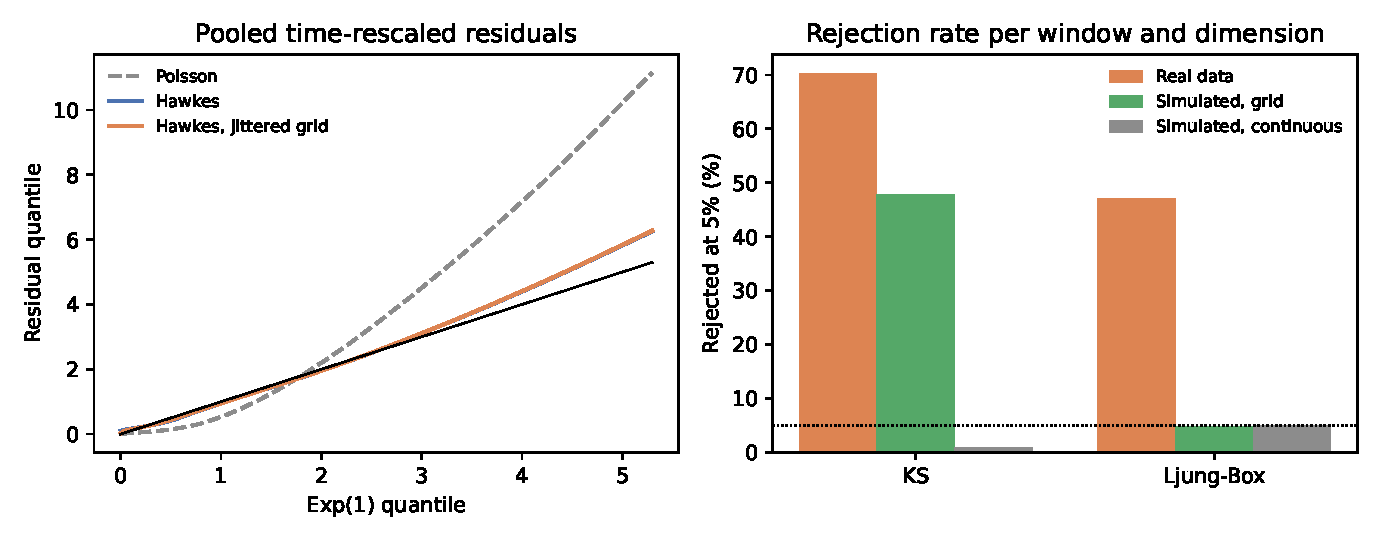
\includegraphics[width=0.9\linewidth]{real_data_residual_diagnostics.pdf}
\caption{Left: Q--Q plot of the pooled time-rescaled residuals of the calibration windows
against $\mathrm{Exp}(1)$. Right: rejection rates on real data and in the two simulated
controls; the dotted line is the nominal 5\%.}
\label{fig:diagnostics}
\end{figure}

The estimates fall far from the synthetic prior (Fig.~\ref{fig:prior}). The median $\beta$
is 2.71 (interquartile range 2.21--3.14), above the prior's upper limit of 2.0, and
$\across$ is below $10^{-3}$ in 89.4\% of the windows. Only 15.4\% of the windows have $\beta$
inside the prior, 0.4\% have a self-excited fraction inside $[0.2,0.8]$, and none satisfies
all ranges at once. Null cross-excitation contrasts with Lee's equity fixed point, where
$\across>\aself$, and agrees with the directional persistence in Table~\ref{tab:data}. Since
a squared-loss estimator approximates the posterior mean under its training prior, the
synthetic networks cannot reach this region.

\begin{figure}[t]
\centering
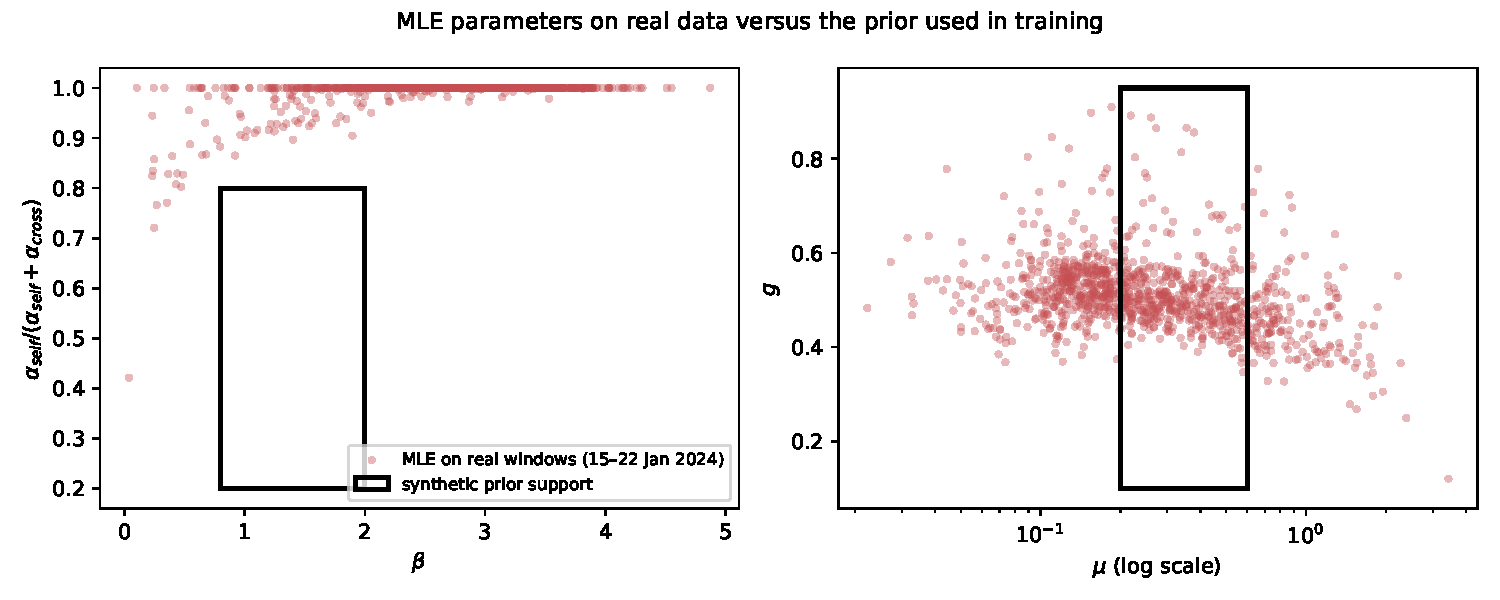
\includegraphics[width=0.9\linewidth]{posthoc_calibracao_vs_prior_en.pdf}
\caption{MLE estimates on the 1,063 calibration windows (points) and the support of the
synthetic training prior (rectangles).}
\label{fig:prior}
\end{figure}

\subsection{Neural estimators on real windows}

Table~\ref{tab:real} reports agreement with the MLE label. Applied as they are, the
synthetic networks are worse than the constant label mean on validation (0.555 and 0.558
against 0.210), with strongly negative $R^2$ for $\aself$ and $\beta$: they shrink into a
prior that does not contain the data. Trained from scratch on 1,063 windows, both improve on
the label mean in validation, but on the test block the LSTM is no better than it (0.250
against 0.218) and the Transformer beats it only modestly (0.169). Fine-tuned from the
synthetic weights, both networks reproduce most of the label
variance, and their test macro MSE is about five times lower than the label mean's. The
fine-tuned LSTM was selected on validation (0.0359 against 0.0413 for the fine-tuned
Transformer); on the test block the Transformer has the lower ensemble MSE (0.0396 against
0.0442), but a post hoc paired comparison per window gives an LSTM-minus-Transformer
difference of 0.0046 with bootstrap 95\% interval $[-0.0020,0.0112]$ and Wilcoxon $p=0.385$:
the two cannot be told apart. The best epochs of the fine-tuned LSTM were 291--299 in every
seed, close to the 300-epoch limit, so its training was cut by the budget.

\begin{table}[t]
\centering
\caption{Agreement with the MLE label on real windows. Validation macro MSE of the
five-seed ensemble and mean $\pm$ SD across seeds; $R^2$ per parameter on validation
relative to the training-label mean; test macro MSE of the ensemble (block opened once).
$^{\ast}$Selected variant.}
\label{tab:real}
\footnotesize
\setlength{\tabcolsep}{4pt}
\begin{tabular}{lrrrrrr}
\toprule
 & \multicolumn{5}{c}{Validation} & Test\\
\cmidrule(lr){2-6}\cmidrule(lr){7-7}
Variant & Ensemble & Seeds & $R^2_{\mu}$ & $R^2_{\aself}$ & $R^2_{\beta}$ & Ensemble\\
\midrule
Training-label mean & 0.2096 & -- & 0.00 & 0.00 & 0.00 & 0.2184\\
LSTM, synthetic weights & 0.5550 & 0.5669 $\pm$ 0.0793 & 0.52 & $-$4.48 & $-$1.19 & 0.2501\\
Transformer, synthetic weights & 0.5575 & 0.5707 $\pm$ 0.0161 & 0.59 & $-$4.63 & $-$1.08 & 0.2747\\
LSTM, from scratch & 0.1385 & 0.1483 $\pm$ 0.0098 & 0.61 & 0.39 & 0.30 & 0.2502\\
Transformer, from scratch & 0.1002 & 0.1060 $\pm$ 0.0012 & 0.93 & 0.50 & 0.47 & 0.1692\\
LSTM, fine-tuned$^{\ast}$ & 0.0359 & 0.0454 $\pm$ 0.0133 & 0.90 & 0.85 & 0.82 & 0.0442\\
Transformer, fine-tuned & 0.0413 & 0.0522 $\pm$ 0.0071 & 0.94 & 0.78 & 0.79 & 0.0396\\
\bottomrule
\end{tabular}
\end{table}

\subsection{Robustness: October 2023}

The October week, never used for training or selection, yields 1,281 windows, and the MLE
converged on all of them. Every variant has a higher loss than on the January test block
(Table~\ref{tab:october}); the error of the label mean nearly triples (0.218 to 0.629), so
the October labels lie farther from the January mean. The fine-tuned networks remain far
ahead, and the zero-shot synthetic networks remain worse than the label mean. The fine-tuned Transformer now has
a lower loss than the selected LSTM (0.083 against 0.121). In the same post hoc paired
comparison, the LSTM-minus-Transformer difference is 0.0384 (bootstrap 95\% interval
$[0.0319,0.0449]$, Wilcoxon $p<10^{-32}$), and the Transformer has the lower loss in 64.3\% of
the windows. Under this change of regime, the fine-tuned Transformer degrades less.

\begin{table}[t]
\centering
\caption{Agreement with the MLE label in the October 2023 robustness window: macro MSE of
the seed ensemble, overall and by tercile of realized volatility. $^{\ast}$Variant selected
on the January validation block.}
\label{tab:october}
\small
\begin{tabular}{lrrrr}
\toprule
Variant & All & Low vol. & Medium vol. & High vol.\\
\midrule
Training-label mean & 0.6292 & 0.4997 & 0.3329 & 1.0550\\
LSTM, synthetic weights & 1.1153 & 1.2838 & 1.2134 & 0.8487\\
Transformer, synthetic weights & 1.0596 & 1.2621 & 1.1169 & 0.7997\\
LSTM, from scratch & 0.4087 & 0.4052 & 0.3289 & 0.4920\\
Transformer, from scratch & 0.3329 & 0.4486 & 0.3120 & 0.2383\\
LSTM, fine-tuned$^{\ast}$ & 0.1212 & 0.1076 & 0.0712 & 0.1849\\
Transformer, fine-tuned & 0.0828 & 0.0343 & 0.0386 & 0.1757\\
\bottomrule
\end{tabular}
\end{table}

\subsection{Hawkes volatility}

Eq.~\eqref{eq:hawkes-vol} is finite in all windows, and its median absolute
log change between consecutive windows (0.097) is close to that of realized volatility
(0.102). Table~\ref{tab:volatility} and Fig.~\ref{fig:volatility} compare the two. With the
MLE, the Hawkes volatility ranks the windows like the realized one (Spearman 0.78 on the
test block at $\Delta=10$~s) and is about 1.27 times higher at horizons of 5 to 30~s. The
ratio falls from about 1.6 at 0.1~s to 1.27 at 10~s: realized variance per unit time grows
with $\Delta$, as expected when successive changes are positively autocorrelated, which is the
persistence that self-excitation describes. Because Eq.~\eqref{eq:hawkes-vol} is a long-run
quantity and the ratio is still about 1.3 at 30~s, either realized variance has not yet
reached its long-run level or the model overstates persistence. With the selected network,
the level is kept but the ranking is largely lost (Spearman 0.28 on the test block): the
network shrinks its estimates toward the training-label mean, compressing the differences
between windows.

\begin{table}[t]
\centering
\caption{Hawkes against realized volatility: median ratio $\sigma_H/\sigma_{RV}$ and
Spearman correlation $\rho_S$ across windows, by sampling interval $\Delta$. ``Network'' is
the selected variant (fine-tuned LSTM ensemble).}
\label{tab:volatility}
\small
\setlength{\tabcolsep}{5pt}
\begin{tabular}{llrrrrrr}
\toprule
 & & \multicolumn{2}{c}{$\Delta=1$ s} & \multicolumn{2}{c}{$\Delta=10$ s}
 & \multicolumn{2}{c}{$\Delta=30$ s}\\
\cmidrule(lr){3-4}\cmidrule(lr){5-6}\cmidrule(lr){7-8}
Block & Parameters & Ratio & $\rho_S$ & Ratio & $\rho_S$ & Ratio & $\rho_S$\\
\midrule
Calibration & MLE & 1.37 & 0.87 & 1.27 & 0.74 & 1.30 & 0.59\\
 & network & 1.39 & 0.56 & 1.30 & 0.40 & 1.34 & 0.36\\
Validation & MLE & 1.36 & 0.79 & 1.24 & 0.67 & 1.27 & 0.51\\
 & network & 1.37 & 0.59 & 1.24 & 0.47 & 1.28 & 0.37\\
Test & MLE & 1.42 & 0.86 & 1.27 & 0.78 & 1.30 & 0.60\\
 & network & 1.56 & 0.34 & 1.38 & 0.28 & 1.45 & 0.33\\
\bottomrule
\end{tabular}
\end{table}

\begin{figure}[t]
\centering
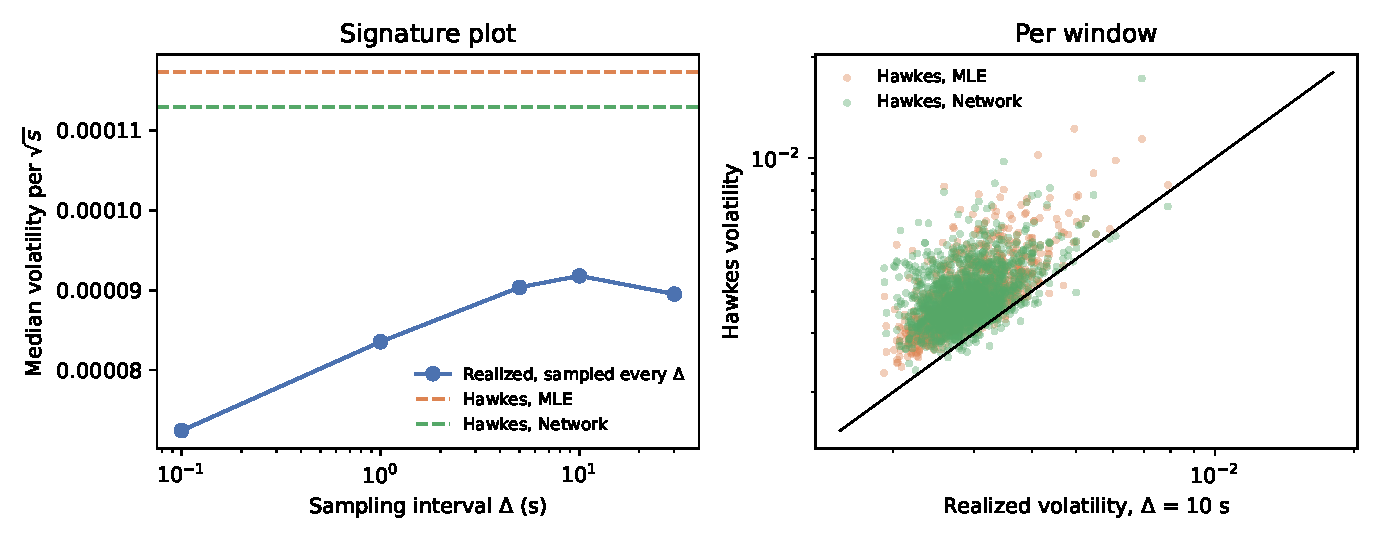
\includegraphics[width=0.9\linewidth]{hawkes_volatility.pdf}
\caption{Calibration and validation windows. Left: median realized volatility per
$\sqrt{\mathrm{s}}$ against the sampling interval (signature plot) and the median Hawkes
level. Right: Hawkes against realized volatility ($\Delta=10$~s) per window.}
\label{fig:volatility}
\end{figure}

\subsection{Robustness of the attention hypothesis to a shift in \texorpdfstring{$\beta$}{beta}}
\label{sec:addendum-beta}

The October result suggests a mechanism: the LSTM may store the decay in its weights, tuned
to the January $\beta$, and degrade faster than the Transformer when $\beta$ moves. We
tested this in an exploratory addendum registered after the main results were frozen, which
does not change them. Hawkes paths were simulated at the centre of the January labels
($\mu=0.23$, $g=0.5$, $\across=0.001$), 400 per value of $\beta$, mapped to the 100~ms grid
exactly as the real data and cut to 1,000 events. The target is each path's MLE, which is
what the fine-tuned networks learned to imitate, and the frozen ensembles are used without
retraining. The registered rule supports the hypothesis if the bootstrap 95\% interval of
the change in the mean LSTM-minus-Transformer loss between $\beta=2.7$ and $\beta=4.5$ lies
above zero.

\begin{table}[t]
\centering
\caption{Mean loss against the MLE on simulated grid paths (ensemble of five seeds,
fine-tuned weights). $^{\ast}$Values added after the registered grid.}
\label{tab:beta}
\small
\setlength{\tabcolsep}{5pt}
\begin{tabular}{lrrrrrrr}
\toprule
True $\beta$ & 1.2 & 2.0 & 2.7 & 3.5 & 4.5 & 6.0$^{\ast}$ & 8.0$^{\ast}$\\
\midrule
Median MLE $\beta$ on the grid & 0.93 & 1.45 & 1.86 & 2.28 & 2.73 & 3.33 & 3.96\\
LSTM & 0.017 & 0.007 & 0.022 & 0.028 & 0.028 & 0.037 & 0.125\\
Transformer & 0.029 & 0.097 & 0.114 & 0.091 & 0.053 & 0.038 & 0.059\\
\bottomrule
\end{tabular}
\end{table}

By the registered rule the hypothesis is supported: the difference grows by 0.067 from
$\beta=2.7$ to $4.5$, with interval $[0.061,0.073]$. Its premise, however, failed
(Table~\ref{tab:beta}). The grid merges events in the same cell and pulls the MLE $\beta$
down, so a true $\beta$ of 4.5 yields a median label of 2.73, the centre of January, not a
shift away from it; on the grid the MLE recovers between 50\% and 80\% of the
continuous-time $\beta$ in this range. In the space of the labels, the LSTM has the lower loss inside and below the January range, where it is the
Transformer that degrades; the two tie near the October median ($\beta\approx3.2$); and above
the training range (95\% of the January labels lie below 3.74) the LSTM's loss grows about
fourfold and crosses the Transformer's. The mechanism therefore holds only for $\beta$ above
the training range, and $\beta$ alone does not explain the October gap, since October also
has larger $\mu$ and $\aself$.

\subsection{How much of the decay does the 100~ms grid hide?}
\label{sec:grid}

The sweep shows that the grid pulls the MLE $\beta$ down. To measure the effect over the
region of the real labels, we simulated 100 continuous-time paths for each $(\mu,\beta)$ of a
mesh ($\mu$ from 0.05 to 2, $\beta$ from 1.2 to 13, $g=0.5$, $\across=0.001$), took them to the
grid, cut them to 1,000 events and fitted the MLE. The median estimate defines a map from
continuous-time parameters to grid labels, which we interpolate in logarithms and invert for
each real window, a form of indirect inference (Table~\ref{tab:grid}).

\begin{table}[t]
\centering
\caption{Median MLE $\beta$ on the 100~ms grid for continuous-time $(\mu,\beta)$, $g=0.5$,
100 paths per cell.}
\label{tab:grid}
\small
\setlength{\tabcolsep}{4pt}
\begin{tabular}{lrrrrrrrrr}
\toprule
$\mu$ $\backslash$ true $\beta$ & 1.2 & 2.0 & 2.7 & 3.5 & 4.5 & 6.0 & 8.0 & 10.0 & 13.0\\
\midrule
0.05 & 1.04 & 1.63 & 2.11 & 2.62 & 3.17 & 3.83 & 4.63 & 5.23 & 5.97\\
0.23 & 0.93 & 1.45 & 1.88 & 2.27 & 2.72 & 3.32 & 4.01 & 4.48 & 5.02\\
1.0 & 0.63 & 0.96 & 1.26 & 1.51 & 1.83 & 2.21 & 2.65 & 2.96 & 3.25\\
2.0 & 0.42 & 0.61 & 0.86 & 0.98 & 1.14 & 1.48 & 1.66 & 1.88 & 1.98\\
\bottomrule
\end{tabular}
\end{table}

The bias grows with $\beta$ and $\mu$, that is, with the share of events that land in an
occupied cell, and the branching ratio is also biased down (to between 0.22 and 0.48), while
$\mu$ is nearly unaffected. Inverted, the median January label of 2.71 corresponds to a
continuous-time $\beta$ of 4.7 (5\%--95\%: 1.9--9.2; 95\% of the windows inside the map): the
grid label is a median 58\% of the continuous value, and the mean memory of an event is about
210~ms rather than 370~ms. October's median of 3.19 corresponds to 6.5. Jittering the times
inside their cell, as in the diagnostics, does not undo this bias, because it breaks ties but
cannot restore merged events. The inversion assumes $g=0.5$ and $\across\approx0$ and gives
the order of magnitude, not a corrected label per window.

\subsection{A better fine-tuning recipe and a fresh test week}
\label{sec:addendum-recipe}

The fine-tuned LSTM reached its best epoch at 291--299 of 300 in every seed, and both
fine-tuned networks predicted $\across$ worse than the label mean because $\beta$ dominates the
loss. Five new arms start from the same synthetic weights with the same data, seeds, learning
rate and batch: a 1,000-epoch cap (LSTM); the cap with a five-epoch warm-up, halving of the
learning rate after ten epochs without improvement and gradient clipping (both networks); and
the latter with a training loss standardized by the variance of each label (both networks).
A sixth candidate, registered before the new week was read, averages the predictions of the
best LSTM and the best Transformer. One candidate is selected on the January validation block
and compared, window by window, with the frozen fine-tuned LSTM on a week never used before:
BTCUSDT and ETHUSDT, 5--11 February 2024, 711 windows labelled by the MLE and read once.

\begin{table}[t]
\centering
\caption{Macro MSE of five-seed ensembles on validation, on the new week and on October 2023
(exploratory).}
\label{tab:recipe}
\small
\begin{tabular}{lrrr}
\toprule
Candidate & Validation & New week & October\\
\midrule
LSTM, fine-tuned (frozen) & 0.0359 & 0.0264 & 0.121\\
Transformer, fine-tuned (frozen) & 0.0413 & 0.0285 & 0.083\\
LSTM, 1,000-epoch cap (selected) & \textbf{0.0294} & 0.0212 & 0.116\\
LSTM, cap + schedule & 0.0358 & 0.0260 & 0.131\\
Transformer, cap + schedule & 0.0448 & 0.0295 & 0.094\\
LSTM, standardized loss & 0.0354 & 0.0315 & 0.102\\
Transformer, standardized loss & 0.0431 & 0.0330 & 0.085\\
Average of LSTM and Transformer & 0.0304 & \textbf{0.0204} & 0.087\\
Mean of the training labels & --- & 0.1826 & 0.629\\
\bottomrule
\end{tabular}
\end{table}

The longer cap was selected on validation (Table~\ref{tab:recipe}); its five seeds stopped at
epochs 158 to 925. On the new week it beats the frozen LSTM by $-0.0052$ (paired bootstrap
95\% interval $[-0.0060,-0.0044]$, Wilcoxon $p<10^{-38}$), with the lower loss in 73\% of the
windows: the original LSTM was undertrained. Among the secondary comparisons (Holm-adjusted),
the average of the two networks also beats the frozen LSTM ($-0.0059$, $p<10^{-12}$) and has
the lowest loss of all; the schedule ties; the standardized loss loses ($+0.005$ and $+0.007$),
although it raises the $R^2$ of $\across$ from $-21$ to $-1.0$ (LSTM) and 0.05 (Transformer),
the only variants not clearly worse than the constant mean on that parameter. No Transformer
arm beats the frozen LSTM on the new week, while in October the Transformers remain the best.
Inside the training regime the LSTM is the better single network, and under a change of regime
the Transformer is more robust. The average, whose two members err in different regions of
$\beta$ (Table~\ref{tab:beta}), has the lowest loss on the new week and is close to the best in
October.

\subsection{A synthetic prior built from the real labels}
\label{sec:scope-b}

The main protocol pretrained on a prior fixed in advance, outside the region of the real
labels. A reduced version of the alternative, registered before any path was generated,
builds the prior from the data. In 75\% of the draws the label of a random training window
is inverted to continuous time by the map of Section~\ref{sec:grid}, with log-normal noise on
$\mu$ and $\beta$ and the branching ratio inflated by 1 to 1.25 to offset the grid; in 25\%
the parameters come from a wide box around the real range. Each of 22,000 paths is simulated
in continuous time, taken to the 100~ms grid, cut to 1,000 events and labelled by the MLE on
the grid, so that the synthetic target means the same as the real one; the real labels fall
inside the 1--99\% synthetic range in 98--99.8\% of the training windows. The LSTM is
pretrained on these paths (150-epoch cap, five seeds) and fine-tuned with the 1,000-epoch
recipe above. Since February had been read, a second unseen week was read once: 4--10 March
2024, 1,860 windows.

\begin{table}[t]
\centering
\caption{Macro MSE of five-seed ensembles with the prior built from the real labels (scope B).
Validation was recorded before March was read; February and October are exploratory.}
\label{tab:scope-b}
\small
\begin{tabular}{lrrrr}
\toprule
Candidate & Validation & March & February & October\\
\midrule
LSTM, fine-tuned (frozen) & 0.0359 & 0.117 & 0.0264 & 0.121\\
LSTM, 1,000-epoch cap & 0.0294 & 0.109 & 0.0212 & 0.116\\
Transformer, fine-tuned (frozen) & 0.0413 & 0.112 & 0.0285 & 0.083\\
Average of the two above & 0.0304 & 0.102 & 0.0204 & 0.087\\
Scope B LSTM, no fine-tuning & 0.1439 & 0.122 & 0.2115 & 0.141\\
Scope B LSTM, fine-tuned & 0.0202 & \textbf{0.040} & 0.0153 & \textbf{0.034}\\
Scope B LSTM + Transformer & \textbf{0.0196} & 0.056 & \textbf{0.0137} & 0.041\\
Mean of the training labels & --- & 0.582 & 0.1826 & 0.629\\
\bottomrule
\end{tabular}
\end{table}

The registered primary comparison, the fine-tuned scope B LSTM against the LSTM with the
1,000-epoch cap on March, is favourable: $-0.068$ (95\% interval $[-0.082,-0.056]$, Wilcoxon
$p<10^{-10}$), a 63\% lower loss, with the lower loss in 72\% of the windows
(Table~\ref{tab:scope-b}). All three secondary comparisons also favour scope B after Holm's
correction, and the sign is the same on February and October. The gain is concentrated where
the earlier networks failed: March and October are the weeks farthest from calibration (the
label mean errs three times more there than on February), and most of the error of the
earlier LSTM is in $\mu$ (March MSE 0.31, $R^2=0.61$), which the scope B network brings to
0.086 ($R^2=0.89$); $\beta$ also improves (0.097 to 0.064). Without fine-tuning the scope B
network is no better than the earlier ones, so the level of the estimates comes from the
fine-tuning. Unlike on February, averaging with the Transformer does not help on
March or October.

\subsection{Can a network undo the grid?}
\label{sec:grid-correction}

The MLE on the grid cannot recover the continuous-time $\beta$, but a network trained on
gridded paths with the true parameters as target can learn the correction. With the protocol
registered before training, the LSTM was trained from scratch on the scope B paths with their
continuous-time parameters as target and compared on 2,000 new paths of the same prior with
the MLE on the grid and the MLE corrected by inverting the map of Section~\ref{sec:grid}.

\begin{table}[t]
\centering
\caption{Error against the continuous-time parameters on 2,000 new simulated paths (median
relative error of $\beta$: signed and absolute).}
\label{tab:grid-correction}
\small
\begin{tabular}{lrrrr}
\toprule
Estimator & Macro MSE & MSE $\beta$ & Bias $\beta$ & $|$Error$|$ $\beta$\\
\midrule
LSTM, trained on the truth & \textbf{0.328} & \textbf{0.90} & $+2.8\%$ & 8.9\%\\
MLE on the grid & 3.951 & 11.68 & $-44.1\%$ & 44.1\%\\
MLE corrected by the map & 0.654 & 1.59 & $-2.4\%$ & \textbf{8.4\%}\\
\bottomrule
\end{tabular}
\end{table}

The network beats the corrected MLE in the registered primary comparison: $-0.326$
(95\% interval $[-0.405,-0.256]$), with the lower loss in 60\% of the paths
(Table~\ref{tab:grid-correction}). The map alone removes almost all of the bias and is the
more precise on a typical path; the network wins through the tails of $\aself$ and $\beta$,
where the map, measured at a single branching ratio, extrapolates poorly. On real windows,
however, the two corrections disagree: the network implies a median continuous-time $\beta$
of 7.7 on validation and 6.3 on February, against 4.9 and 3.1 from the map (Spearman 0.55).
The real windows are not Hawkes paths, so a correction learned in simulation does not transfer
safely, and without the continuous-time truth neither can be checked.

\subsection{Hawkes volatility with the addendum networks}
\label{sec:vol-addendum}

Applied post hoc to February (711 windows), with the comparison registered before computing
it, the Hawkes volatility of the LSTM+Transformer average ranks windows like realized
volatility with Spearman 0.63, against 0.47 for the frozen LSTM (difference 0.155, bootstrap
95\% interval $[0.130,0.181]$); the Transformer alone reaches 0.69 and the MLE 0.77. Training
the LSTM for longer barely helps (0.49). All estimators get the level right (median ratio
1.3--1.4). The LSTM has the lower parameter error, but the Transformer preserves more of the
differences between windows, on which the ranking depends.

%% ===========================================================================================
\section{Discussion}
\label{sec:discussion}

\subsection{The hypotheses}

\emph{H1 is supported as to structure and volume.} The public data yield sequences with the
structure of Lee's inputs in sufficient volume. Their content differs from equities, however:
persistent direction, multi-tick jumps and times discretized by the grid.

\emph{H2 is partially supported.} The LSTM's error is of the same order as the MLE's (0.0111
against 0.0103 at the fixed point; practically equal median per-path loss on the synthetic
test). The substantially lower latency is not confirmed at batch size one against an
efficient MLE; it holds for batched inference.

\emph{H3 is not supported on synthetic data.} The Transformer did not reduce error: its mean
macro MSE was higher, without significance across seeds, and its ensemble lost to the LSTM's
path by path in every regime, including the near-critical one. Its advantages were latency
on MPS (5~ms against 30~ms) at the cost of 2.7 times longer training. On real windows, the
fine-tuned architectures cannot be told apart on the test
block, and in October the Transformer has the lower loss in 64\% of the windows. This is the
only evidence in favour of H3, and it comes from a post hoc comparison rather than the
pre-registered selection. The $\beta$ sweep (Section~\ref{sec:addendum-beta}) does not
explain it by a shift in $\beta$ alone. On a pre-registered new week no Transformer arm beat
the frozen LSTM, but the average of the two did (Section~\ref{sec:addendum-recipe}), so attention
helped as a complement to the LSTM. That complement depends on the prior: once the
LSTM is pretrained on a prior built from the real labels (Section~\ref{sec:scope-b}), it is
the best estimator on March and October by itself, and the average no longer helps. The
Transformer keeps one advantage, for volatility: it preserves more of the ranking of windows
(Section~\ref{sec:vol-addendum}).

\subsection{Why the networks win on aggregate MSE}

The MLE's synthetic macro MSE is about 25 times the networks', but the gap has two sources,
neither of which is greater accuracy on a typical path. The first is identifiability: with low
$g$ the MLE returns extreme values of $\beta$ that legitimately maximize the likelihood. The
second is the prior: the networks approximate the posterior mean under the training
distribution and never leave its range, which bounds their worst case at the price of
shrinkage bias. This robustness holds only if the prior represents the data,
which is not the case on crypto. Lee's qualitative conclusions survive (error of the same order as
the MLE, shrinkage, a nearly unbiased MLE at a well-identified point); absolute MSE values
are not comparable across the two studies because they depend on parameter ranges that the
paper does not publish. Two points diverge: the speed gain of two orders of magnitude, which
a double-sum likelihood recovers (Table~\ref{tab:cost-variants}), and the use of aggregate MSE
alone, which hides identifiability failures that initialization at
the true value tends to mask.

\subsection{What the real data show}

Price changes in these contracts cluster strongly, but a single
exponential kernel does not capture all of the clustering, and the grid explains part, not all, of the
departure from $\mathrm{Exp}(1)$. On real data the target of the networks is therefore the
MLE of an approximating model, observed through the grid, whose label is about 58\% of the
continuous-time decay rate (Section~\ref{sec:grid}). Its parameters ($\across\approx0$, $\beta\approx2.7$) lie
outside the synthetic prior, so synthetic training does not transfer directly; it is useful
as an initialization, since only fine-tuned networks explain most of the label variance with
1,063 training windows. The reduced scope B shows the effect of the prior: a prior
built from the real labels and simulated on the grid cuts the out-of-sample loss by almost
two thirds, mostly by extrapolating $\mu$ to activity levels the calibration week did not
cover. For volatility, reproducing the label on average is not enough: the selected network
keeps the level of the Hawkes volatility but loses most of the cross-sectional ranking that
the MLE preserves; the Transformer recovers much of it, but not all.

\subsection{Limitations and threats to validity}

\emph{Construct.} On real data the label is the MLE of a model that the residual tests reject
in part, and $\across$ lies on the boundary of the parameter space, where the usual asymptotic
theory does not hold; the labels are biased by the grid, which jittering does not undo and which a network
trained on the truth corrects only in simulation.
\emph{Prior.} The synthetic metrics depend on ranges that were not
calibrated on the data; the reduced scope B, which calibrates them, was run for the LSTM only
and with a single prior design. \emph{Statistical.} Five seeds capture only part of training
variability; one synthetic LSTM seed and all fine-tuned LSTM seeds were limited by the
300-epoch budget, which the addendum confirms; the comparison between fine-tuned networks on the test and October blocks
is post hoc. \emph{Architecture.} Neither network was tuned, the batch sizes differ (64
against 8), and the post-LN Transformer was trained without warm-up. \emph{Internal.} Leakage
across windows and tuning on test data are mitigated by chronological splits and a test
block locked behind an explicit flag and opened once. \emph{External.} Two assets, one venue
and two months do not represent the market; the empirical test block covers three days,
including a weekend. \emph{Computational.} Latency depends on hardware, batch size, warm-up
and contention between processes.

%% ===========================================================================================
\section{Conclusion}
\label{sec:conclusion}

We reproduced the qualitative findings of \citet{lee2023} at the published parameter point
and compared the paper's LSTM with a Transformer encoder under a frozen protocol on public
cryptocurrency data. On synthetic data, attention brought no gain in accuracy. The networks'
advantage over the MLE in aggregate MSE comes from robustness on weakly identified paths and
from shrinkage toward the prior; on a typical path the MLE is equally accurate and, when
implemented efficiently, equally fast at batch size one. On BTCUSDT and ETHUSDT perpetual
futures, the Hawkes model captures most but not all of the clustering, with parameters in a
different region from equities and no cross-excitation. Networks reproduce the MLE on real
windows only when fine-tuned from synthetic weights; fine-tuned, the LSTM and the Transformer
are equivalent on the test block, and the Transformer degrades less in a different month. On
a pre-registered new week, the LSTM trained for longer and the average of the two networks
both beat the selected LSTM, the average by the widest margin; on a second new week, an LSTM
pretrained on a prior built from the real labels cut the loss by almost two thirds. The
answer to the research question is negative for accuracy on synthetic data and open for
robustness on real data.

Natural next steps are to extend the prior built from the real labels to the Transformer and
to more weeks and assets; to make the grid correction trustworthy on real data, with a
grid-aware likelihood \citep{lambe2025} and a prior that covers the misspecification of the
market; to replace the single exponential kernel, as the residual dependence
suggests; to tune both architectures without touching any test block and to confirm the
October result on a pre-registered week outside the training regime; and to train directly for volatility with a
loss that preserves the ranking of windows.

\section*{Data and code availability}

The market data are public (Binance Public Data). The code, configuration files, decision
records and generated tables are kept in the project repository; the numbers in this paper are
taken from tables generated by script from the saved artifacts. % TODO: add repository URL once public.

\appendix

\section{Reproduction ambiguities in \texorpdfstring{\citet{lee2023}}{Lee (2023)}}
\label{app:lee}

The paper mentions paths of 2,000 steps but an input shape of 1,000; our protocol fixes
1,000 events and does not compare lengths. It does not publish the parameter ranges, seeds,
batch size or the NBBO data. It calls the two LSTM layers followed by a dense layer ``three
layers''; our implementation follows that structure. The $\log(1+\Delta t)$ input and the
$\pm1$ direction encoding are our reconstructions (Lee uses inter-arrival times and types
1/2). All such decisions are marked R2 in the project records.

\renewcommand{\bibfont}{\small}
\bibliographystyle{elsarticle-harv}
\bibliography{references}

\end{document}
